\chapter{Experimentos}\label{chapter:implementation}

\par La implementaci\'on del algoritmo de reconocimiento de patrones propuesto se realiz\'o en el lenguaje de programaci\'on Python [\cite{22}]. La raz\'on principal: el conjunto de bibliotecas que incluye, tanto para la resoluci\'on del sistema de ecuaciones, como para determinar la transformada wavelet de un vector, lo mismo en $L^2(\mathbb{Z}_N)$ que en $L^2(\mathbb{Z}_{N_1}\times\mathbb{Z}_{N_2})$.

\par El programa se descompone en dos algoritmos y cada algoritmo en dos partes, es decir: un primer algoritmo para la detecci\'on de patrones unidimensionales en una se\~nal y un segundo para detectar un patr\'on de dimensiones cuadradas en una imagen o mamograf\'ia. En la primera fase de cada algoritmo, se plantea el sistema de ecuaciones cuya soluci\'on es el filtro de paso alto y se le da soluci\'on empleando el m\'etodo num\'erico que se mostrar\'a a continuaci\'on, mientras que en la segunda fase, se toma la wavelet creada a partir del banco de filtro con el vector hallado y se determina la transformada de la imagen de muestra (la cual no necesita ser cuadrada), tras la cual se obtienen las cuatro matrices o im\'agenes mencionadas anteriormente; de ellas se analiza la martiz $cD$ en busca de valores cercanos a cero con la funci\'on de similaridad $\mathbb{S}$ y se seleccionan los mejores candidatos de ocurrencia del patr\'on.\\

\par El problema principal del algoritmo es la resoluci\'on del sistema de ecuaciones no lineales. Por lo que se analizar\'a primero este punto antes de entrar en la implementaci\'on del programa en general.\\

\section{M\'etodos para resolver sistemas de ecuaciones no lineales}

\par Para la resoluci\'on del sistema no lineal, se consideraron varios m\'etodos num\'ericos tales como: Newton, Cuasi-Newton, descenso por gradiente, Runge-Kutta y otro empleado para la resoluci\'on de modelos de optimizaci\'on. Se analizar\'an cada uno de ellos y se determinar\'a cu\'al producir\'ia un resultado m\'as cercano al que se desea obtener.

\subsection{M\'etodo de Newton}

\par En el caso del m\'etodo de Newton [\cite{23}], consiste en un algoritmo iterativo, que en cada iteraci\'on actualiza el valor $x_0$ inicial y el jacobiano del sistema, a fin de que $x_0$ siempre se encuentre en una vecindad cada vez m\'as cercana de la ra\'iz del sistema. Este m\'etodo es muy efectivo en peque\~nos sistemas de ecuaciones y converge r\'apidamente en caso de que se tome un valor inicial relativamente cercano a la ra\'iz. Sin embargo, el problema anteriormente planteado no entra dentro de dichos sistemas de ecuaciones, ya que la dimensi\'on de los vectores que se usar\'an para el filtro pueden ser bastante grandes, por lo que la posibilidad de encontrar un primer valor $x_0$ cercano a la ra\'iz se hace muy peque\~na y en muchos casos el algoritmo podr\'ia no converger.\\

\par La Figura 3.1 muestra la efectividad del m\'etodo de Newton para distintas dimensiones del sistema de ecuaciones.

\begin{figure}[h]
\center
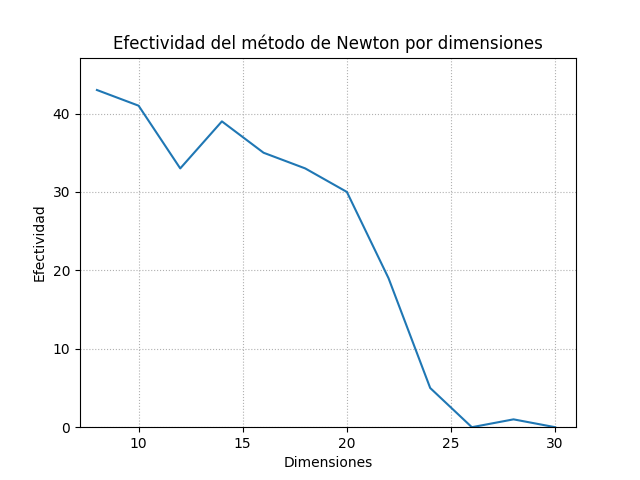
\includegraphics[scale=.45]{Graphics/Newton.png}
\caption{Efectividad (\%) del m\'etodo de Newton en el modelo para un aumento de la dimensi\'on.}
\end{figure}

\par Durante el experimento, se ejecut\'o el m\'etodo $100$ veces por cada dimensi\'on y se determin\'o el valor de la efectividad, dada el porciento que representa la cantidad de casos en los cuales el algoritmo converge satisfactoriamente, del total de casos. Como se puede apreciar, con este m\'etodo se pueden obtener valores correctos hasta con sistemas de dimensi\'on $N=26$, aunque para estos \'ultmos valores la posibilidad de encontrarlos es muy baja.

\subsection{M\'etodo Cuasi-Newton}

\par Por otro lado, el m\'etodo Cuasi-Newton [\cite{23}] constituye una mejora del m\'etodo de Newton en el sentido de que no es necesario hallar en cada iteraci\'on la inversa del jacobiano del sistema, sino que utiliza una matriz definida positiva para aproximar la inversa de la matriz hessiana, simplificando de esta forma el proceso. Sin embargo, como el m\'etodo de Newton, requiere un valor inicial $x_0$ cercano a la ra\'iz para converger.

\par Usando el mismo experimento que en el m\'etodo de Newton, se tomaron $100$ patrones aleatorios para cada dimensi\'on y se determin\'o la efectividad del m\'etodo Cuasi-Newton Broyden-Fletcher-Goldfarb-Shanno (BFGS). La Figura 3.2 muestra los resultados del an\'alisis.\\

\begin{figure}[h]
\center
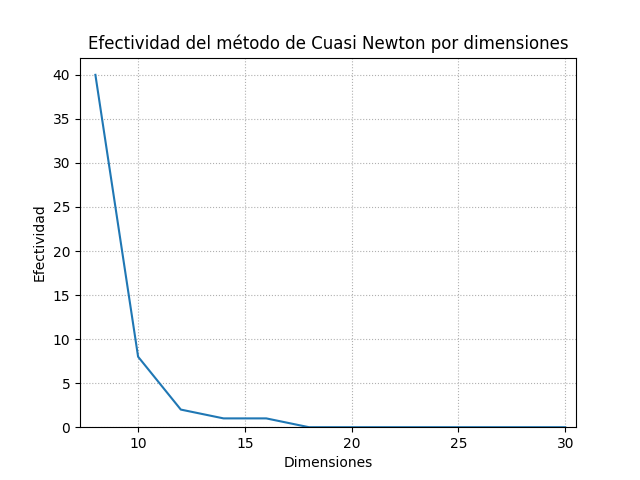
\includegraphics[scale=.4]{Graphics/CuasiNewton.png}
\caption{Efectividad (\%) del m\'etodo Cuasi-Newton en el modelo para un aumento de la dimensi\'on.}
\end{figure}

\par Como puede apreciar, inicialmente tiene una efectividad del $40\%$ para un sistema de dimensi\'on $8$, sin embargo, con un aumento de esta, comienza a reducir hasta que, a partir de $N=18$ se vuelve inefectivo.

\subsection{M\'etodo de Descenso por Gradiente}

\par El m\'etodo del descenso por gradiente [\cite{23}] es un m\'etodo usado para la determinaci\'on de m\'inimos, por lo tanto, para usar este m\'etodo fue necesario trabajar con la norma de del vector formado por las ecuaciones del sistema, de esta forma el valor $x$ que minimice la norma constituye la ra\'iz en el sistema original. La idea de optimizaci\'on de este m\'etodo, es usar la direcci\'on contraria al gradiente en el punto actual como direcci\'on de b\'usqueda, moverse una distancia $\alpha$ y volver a repetir la operaci\'on. A medida que vaya acerc\'andose al m\'inimo, la distancia $\alpha$ se reduce y m\'as lenta es la convergencia. El problema fundamental de este m\'etodo es que puede converger a m\'inimos locales, muy lejos de la ra\'iz verdadera del sistema y esto podr\'ia traer dificultades a la hora de detectar el patr\'on.\\\

\par La Figura 3.3 muestra la efectividad de este m\'etodo para $12$ valores de dimensiones distintas.\\

\begin{figure}[h]
\center
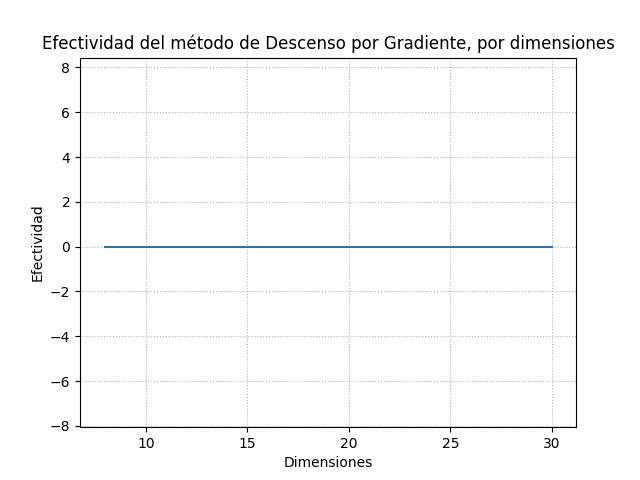
\includegraphics[scale=.45]{Graphics/DescensoGradiente.png}
\caption{Efectividad (\%) del m\'etodo de descenso por gradiente en el modelo para un aumento de la dimensi\'on.}
\end{figure}

\par Aunque al compararlo con los primeros m\'etodos vistos, r\'apidamente ser\'ia descartado, puede ser \'util como un m\'etodo de aproximaci\'on inicial.

\subsection{M\'etodo de Runge-Kutta}

\par El pr\'oximo m\'etodo es el de Runge-Kutta [\cite{23}]. Este es un m\'etodo num\'erico que, al igual que el m\'etodo de Newton, usa el jacobiano del sistema. M\'as a\'un, 
los m\'etodos de Runge Kutta son generalizaciones de la f\'ormula de Euler:
\begin{eqnarray}
x_{i+1}=x_{i}+hf(t_i,x_i),\nonumber
\end{eqnarray}
donde el valor de $f$ es reemplazado por un promedio ponderado de valores de $f$ en el intervalo $t_i\leq t \leq t_{i+1}$. Es decir,
\begin{eqnarray}
x_{i+1}=x_i+h(w_1k_1+w_2k_2+...+w_mk_m).\nonumber
\end{eqnarray}
En este caso se usar\'a Runge-Kutta de orden 4. Realizando el mismo experimento que con los m\'etodos anteriores, se obtiene el resultado mostrado en la Figura 3.4.\\

\begin{figure}[h]
\center
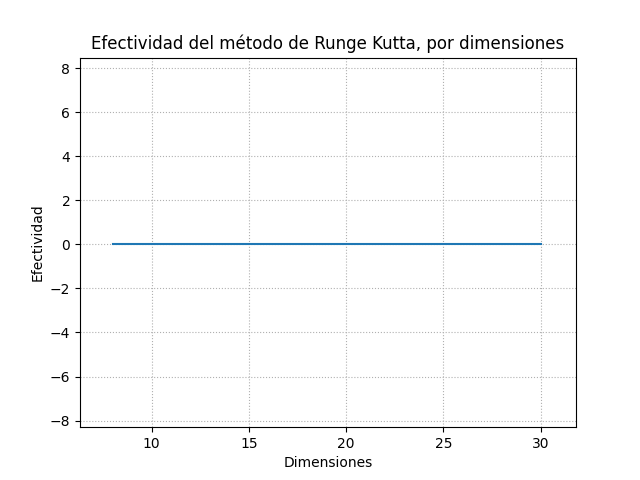
\includegraphics[scale=.4]{Graphics/RungeKutta.png}
\caption{Efectividad (\%) del m\'etodo de Runge-Kutta en el modelo para un aumento de la dimensi\'on.}
\end{figure}

\subsection{Gekko}

\par El \'ultimo m\'etodo que se analizar\'a constituye un m\'etodo usado para la resoluci\'on de problemas de maximizaci\'on y minimizaci\'on de funciones. Como parte de las bibliotecas de Python, se encuentra \textit{gekko} [\cite{13}]. \textit{Gekko} es un paquete de optimizaci\'on y aprendizaje autom\'atico que usa diferenciaci\'on autom\'atica y algoritmos basados en gradientes como APOPT (Advanced Process OPTimizer) [\cite{25}] o IPOPT (Interior Point OPTimizer) [\cite{26}] para encontrar soluci\'on a problemas de optimizaci\'on. Si cada ecuaci\'on constituye una restricci\'on y se considera la norma de las restricciones como la funci\'on objetivo, entonces es posible transformar el sistema de ecuaciones no lineales en un modelo de optimizaci\'on no lineal. Al usar \textit{gekko} para resolver los sistemas con distintas dimensiones, se obtienen los datos mostrados en la Figura 3.5.\\

\begin{figure}[h]
\center
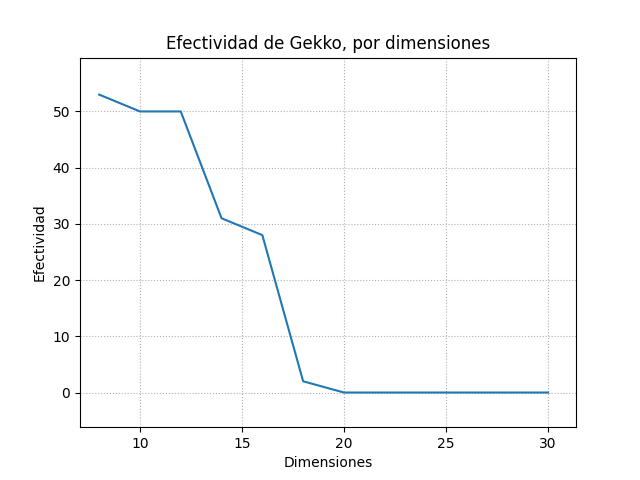
\includegraphics[scale=.4]{Graphics/Gekko.png}
\caption{Efectividad (\%) del m\'etodo de Gekko en el modelo para un aumento de la dimensi\'on.}
\end{figure}

\par En comparaci\'on con los primeros dos m\'etodos, aunque a partir de un valor de dimensi\'on dado se vuelve ineficiente, muestra un comportamiento con valores de efectividad muy buenos en comparaci\'on con el m\'etodo Cuasi-Newton pero inferiores a los de Newton.

\subsection{Mejores Resultados}

\par Hasta el momento se han analizado los m\'etodos por separado, de los cuales el m\'etodo de Newton a dado los mejores resultados. Tal como se mencion\'o varios de ellos dependen de una buena aproximaci\'on inicial. Dado que el m\'etodo del descenso por gradiente y Runge-Kutta no entran dentro de estos, se usar\'an para lograr una buena aproximaci\'on inicial y, posteriormente, aplicar alguno de los otros m\'etodos propuestos. Realizando nuevamente el experimento, usando cada m\'etodo de aproximaci\'on inicial con cada m\'etodo para encontrar la ra\'iz del sistema, se obtienen los resultados mostrados en la Figura 3.6.\\

\begin{figure}[h]
  \begin{center}
    \subfigure[\begin{scriptsize}
        Descenso por Gradiente y Newton
        \end{scriptsize}]{
        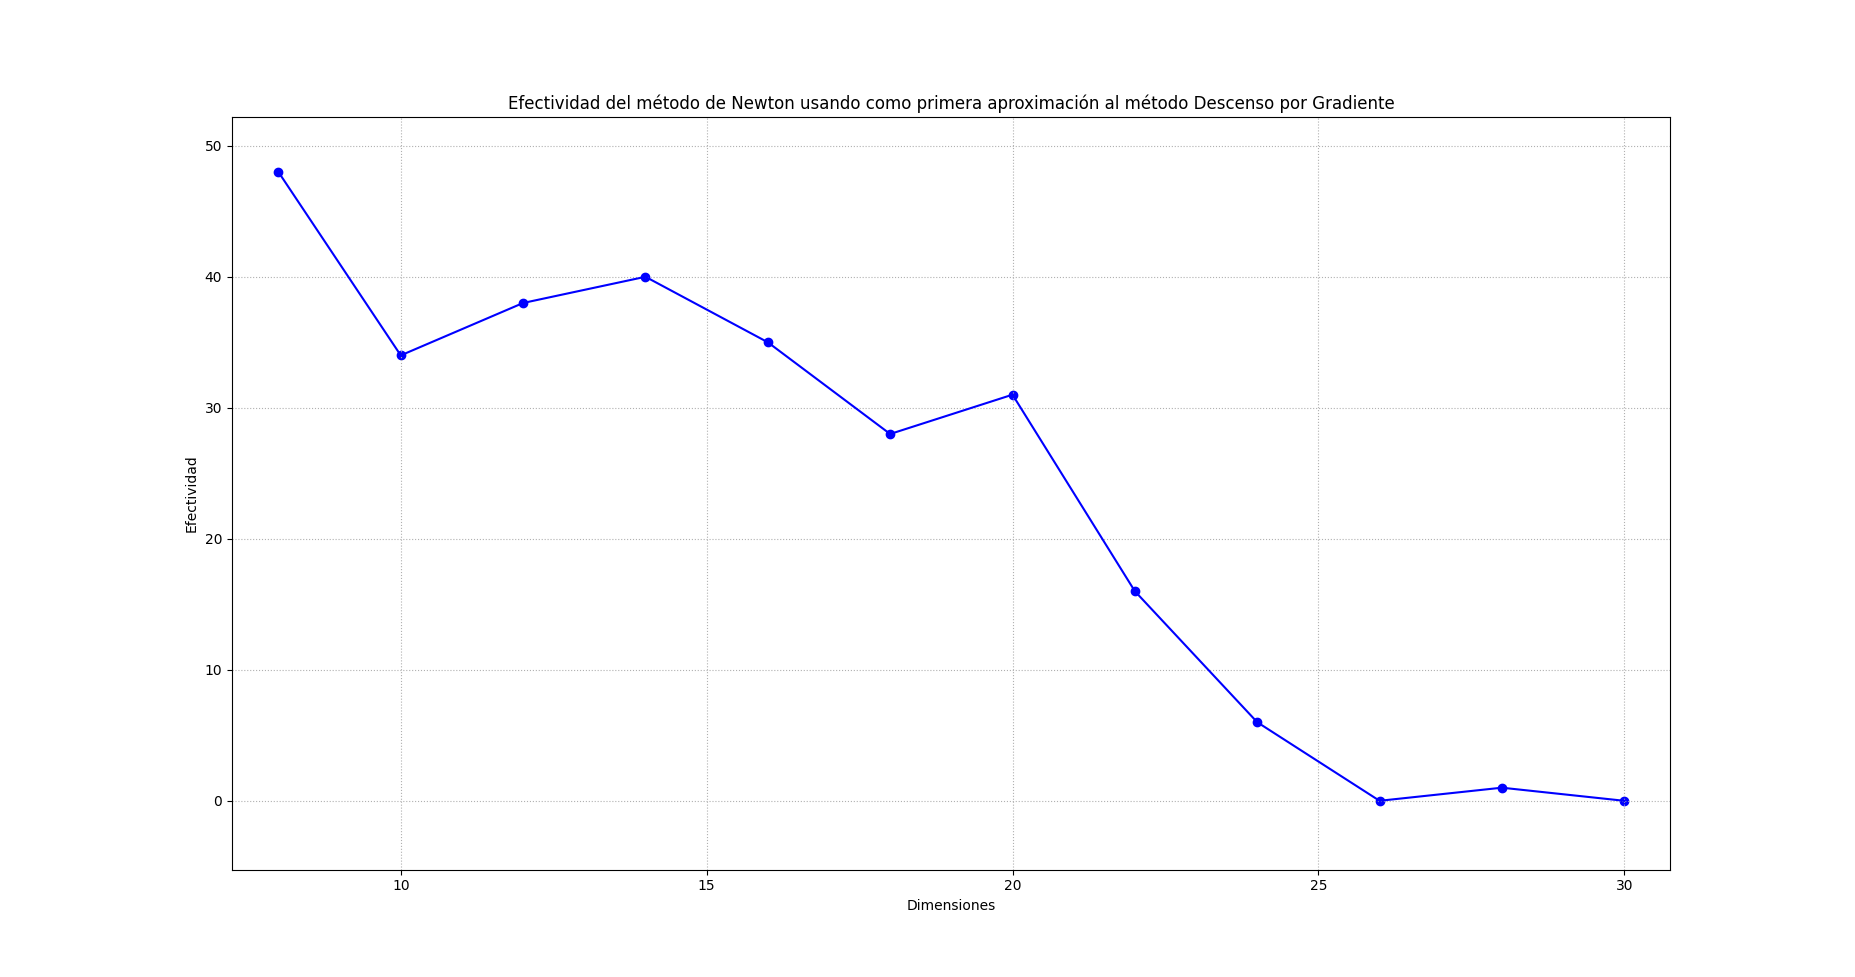
\includegraphics[width=.45\textwidth]{Graphics/GD_N.png}
        \label{GD-N}}
    \subfigure[\begin{scriptsize}
	    Runge-Kutta y Newton
        \end{scriptsize}]{
        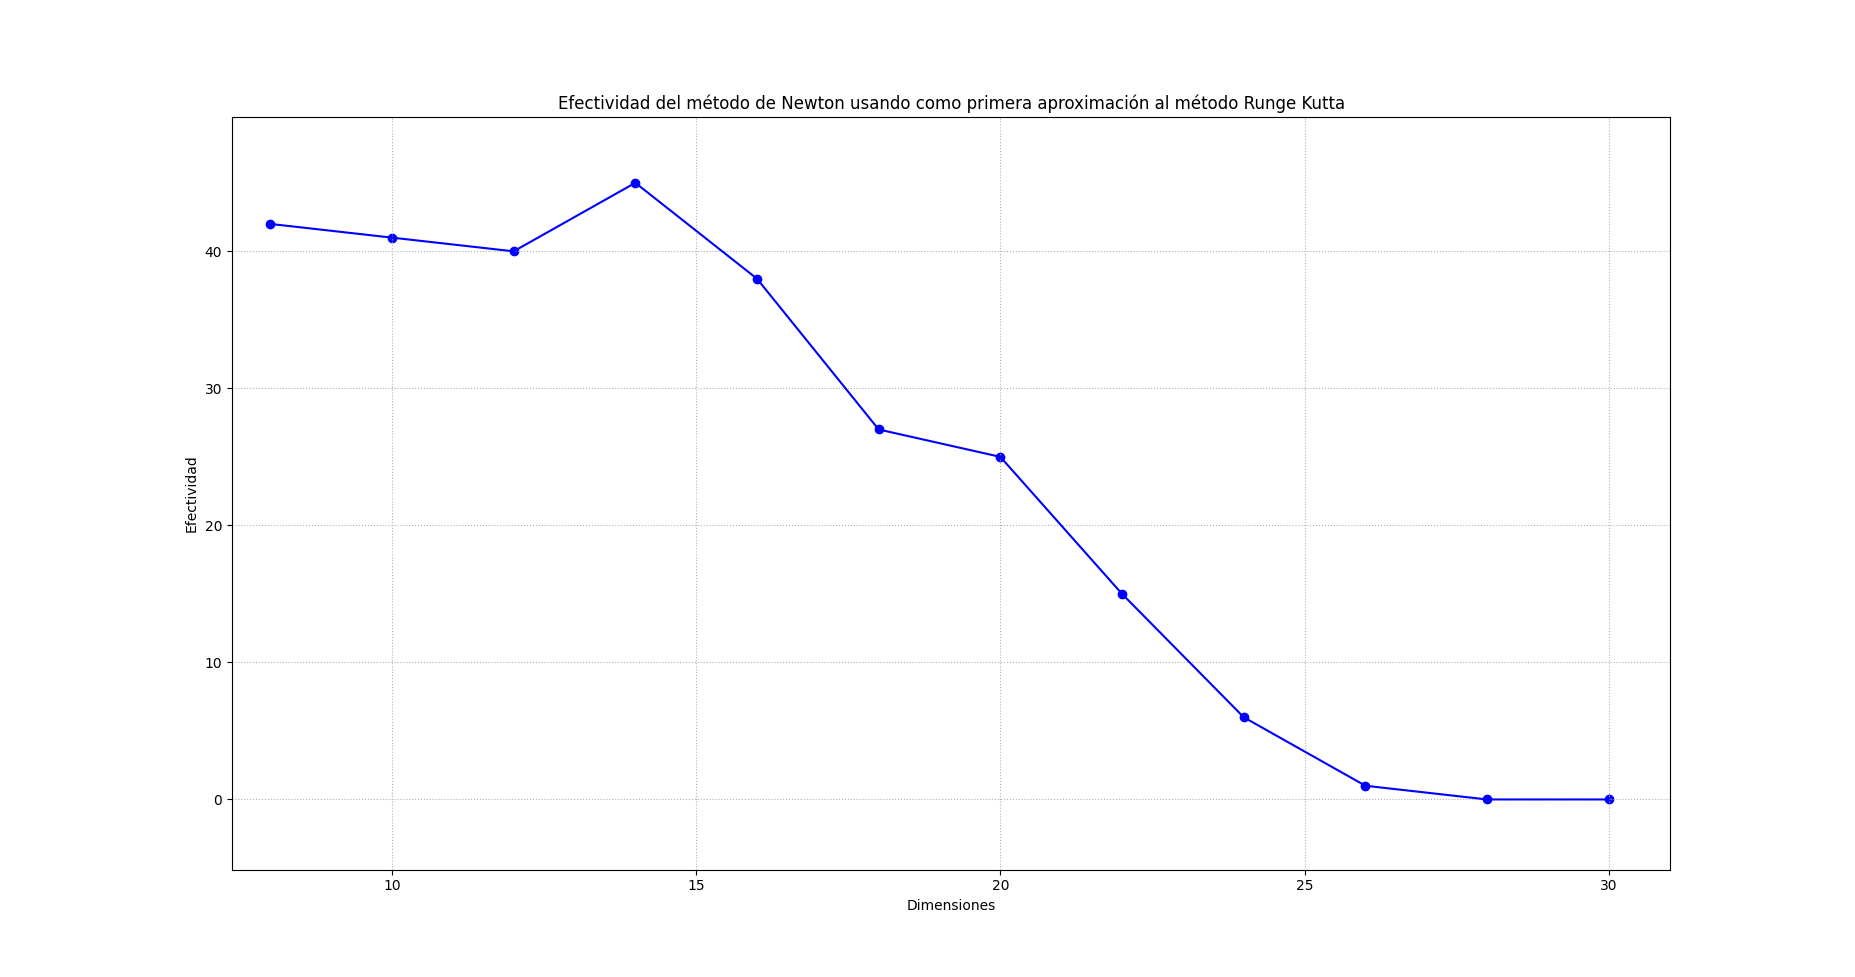
\includegraphics[width=.45\textwidth]{Graphics/RK_N.png}
        \label{RK-N}}
    \subfigure[\begin{scriptsize}
        Descenso por Gradiente y Cuasi-Newton
        \end{scriptsize}]{
        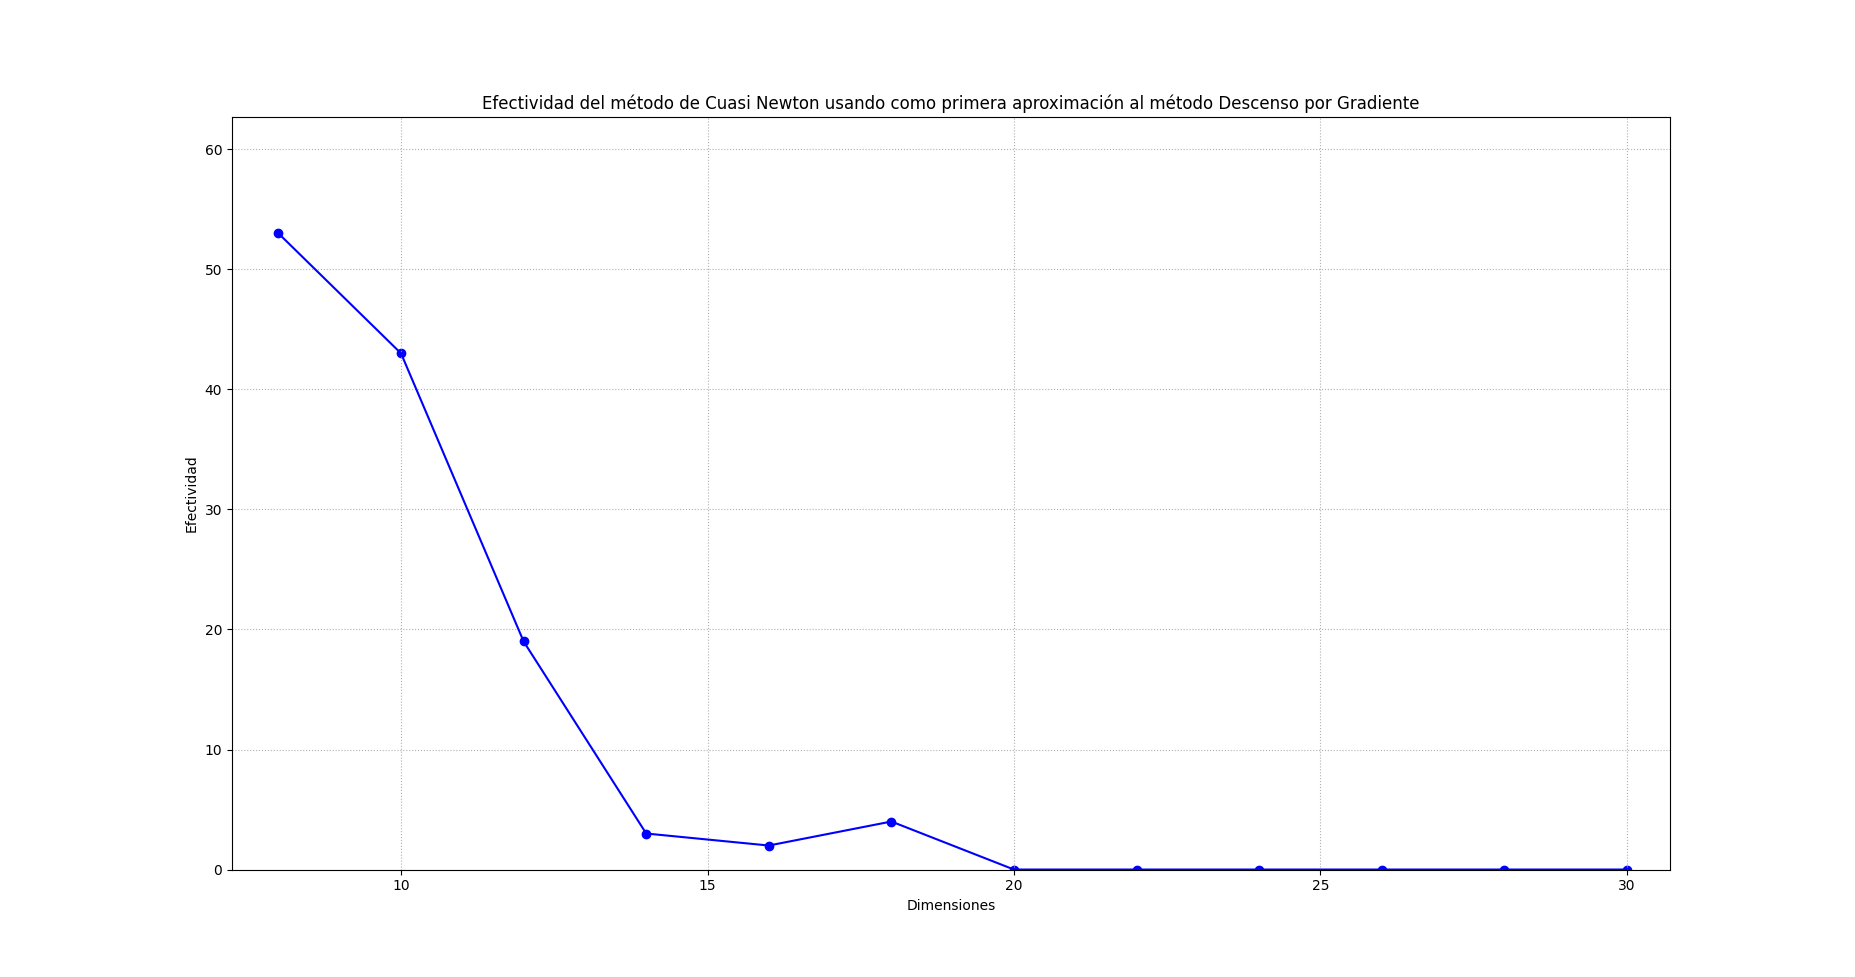
\includegraphics[width=.45\textwidth]{Graphics/GD_CN.png}
        \label{GD-CN}}
    \subfigure[\begin{scriptsize}
        Runge-Kutta y Cuasi-Newton
        \end{scriptsize}]{
        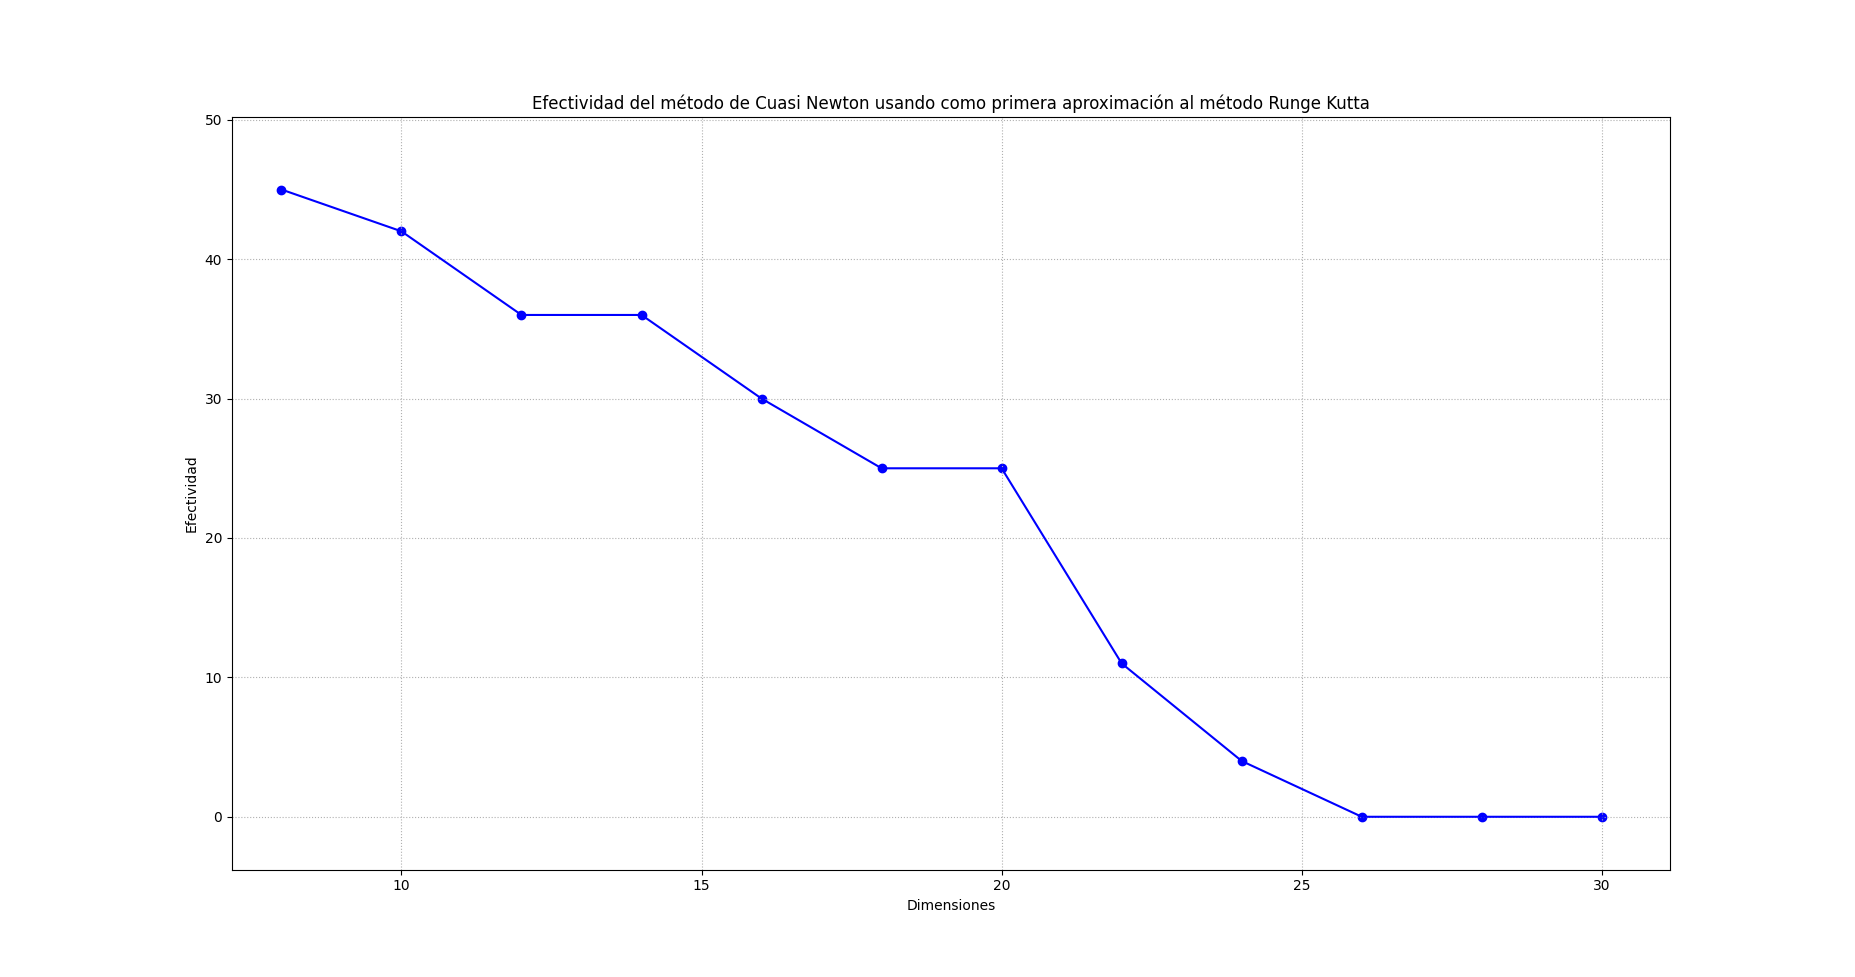
\includegraphics[width=.45\textwidth]{Graphics/RK_CN.png}
        \label{RK-CN}}
    \subfigure[\begin{scriptsize}
        Descenso por Gradiente y Gekko
        \end{scriptsize}]{
        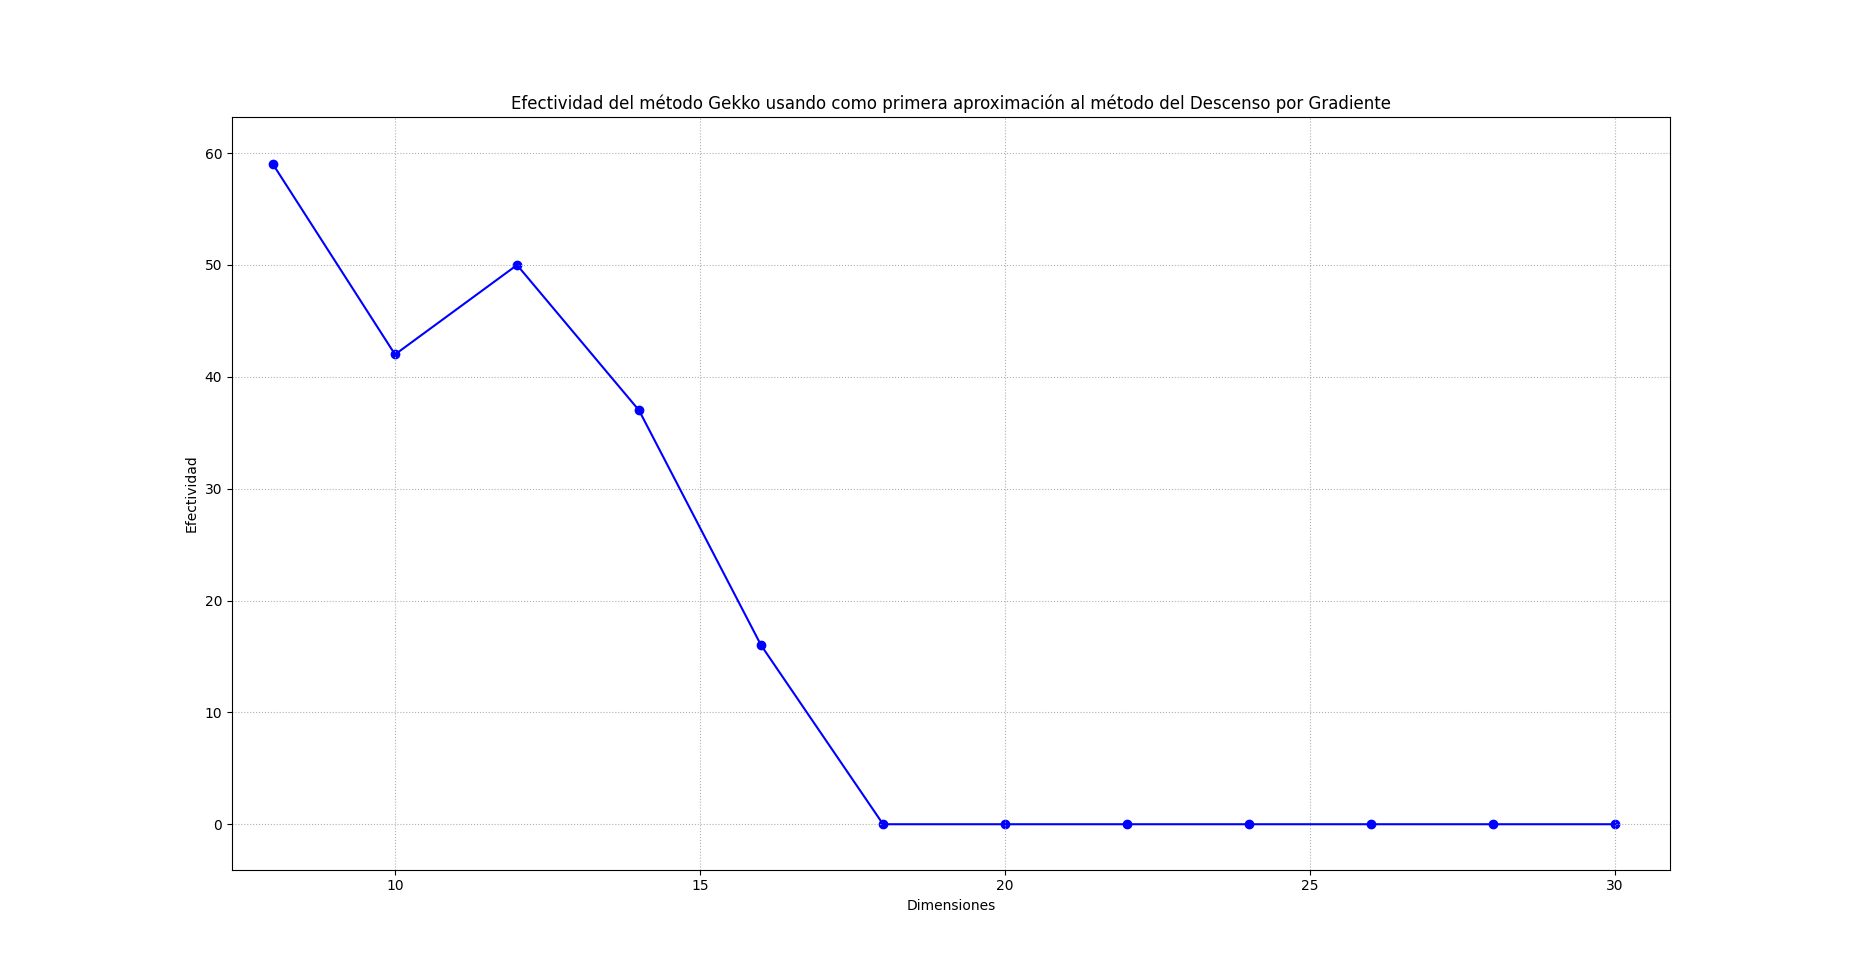
\includegraphics[width=.45\textwidth]{Graphics/GD_Gekko.png}
        \label{GD-G}}
    \subfigure[\begin{scriptsize}
        Runge-Kutta y Gekko
        \end{scriptsize}]{
        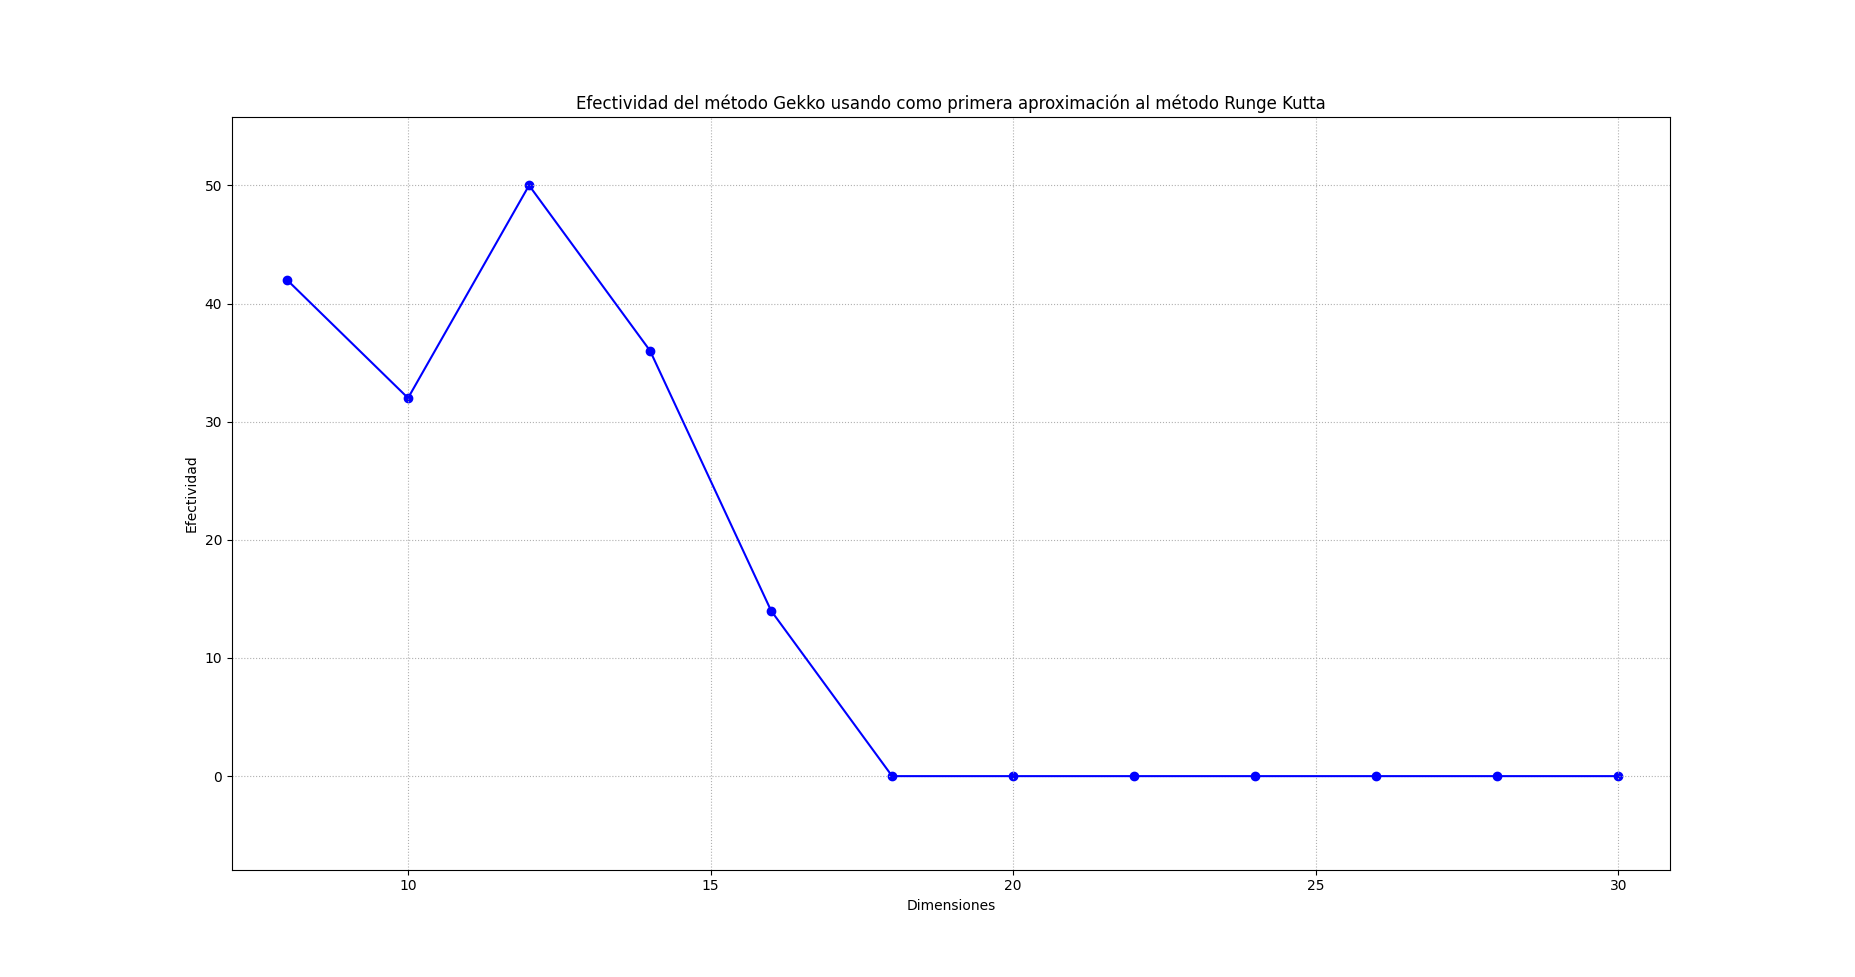
\includegraphics[width=.45\textwidth]{Graphics/RK_Gekko.png}
        \label{RK-G}}
    \caption{Resultados obtenidos empleando los m\'etodos del Descenso por Gradiente y Runge-Kutta para encontrar una aproximaci\'on inicial y, los m\'etodos Newton, Cuasi-Newton y Gekko para resolver el sistema.}
    \label{metodos-combinados}
  \end{center}
\end{figure}

\par Seg\'un los resultados mostrados, Newton con aproximaci\'on inicial a Runge-Kutta constituye la combinaci\'on de m\'etodos con mayor compatibilidad con el sistema propuesto y, por consiguiente, la combinaci\'on que se usar\'a para determinar los filtros de las shapelets, al menos para el caso de una dimensi\'on.\\

\section{Algoritmo de reconocimiento en una dimensi\'on}

\par Una vez se tiene la se\~nal del patr\'on, el primer paso es definir el sistema de ecuaciones a partir del mismo y resolverlo aplicando los m\'etodos de Runge-Kutta y Newton. Al resolver el sistema se obtienen los valores de las componentes del primer vector (llam\'emoslo $v$). A partir de $v$ se construyen los vectores $u$, $\tilde{u}$ y $\tilde{v}$ siguiendo las definiciones dadas en la secci\'on 1.1.1. Con estos cuatro vectores, se construye el banco de filtros y con \'el la wavelet. Para ello, se emplea la biblioteca \textit{PyWavelets} [\cite{27}] de Python, con la cual es posible crear una wavelet recibiendo como par\'ametro el banco de filtros (ver c\'odigo 3.1):\\

\begin{lstlisting}[caption=Creaci\'on de una wavelet a partir del banco de filtros]
shapelet = pywt.Wavelet(filter_bank = [u_, v_, u, v])
\end{lstlisting}

\par El siguiente paso es tomar una se\~nal en la cual se quiere determinar si el patr\'on est\'a o no presente, y aplicar la transformada de wavelet usando la wavelet creada con el filtro:\\

\begin{lstlisting}[caption=C\'alculo de la transformada discreta de Wavelet usando pywt]
cA, cD = pywt.dwt(signal, shapelet)
\end{lstlisting}

para posteriormente determinar, seg\'un los valores cercanos a cero de $cD$, la presencia del patr\'on en la se\~nal.

Consid\'erese el caso de ejemplo de la secci\'on 1.1.3:
\begin{eqnarray}
m=(0.2,0.5,0.45,0.85,0.8,-0.75,0.25,0.2,0.55).\nonumber
\end{eqnarray}

\par Tras construir el sistema y resolverlo se obtiene como una de las posibles soluciones:

\begin{eqnarray}
v=(0.0445, 0.4373, 0.1074, -1.6020, 1.0664, -0.2296, 0.1959, -0.0199),\nonumber
\end{eqnarray}

mientras que:

\begin{eqnarray}
u&=&(0.4373, -0.0445, -0.0199, 0.1959, -0.2296, -1.0664, -1.6020, -0.1074),\nonumber\\
\tilde{v}&=&(0.0445, -0.0199, 0.1959, -0.2296, 1.0664, -1.6020, 0.1074, 0.4373),\nonumber\\
\tilde{u}&=&(0.4373, -0.1074, -1.6020, -1.0664, -0.2296, -0.1959, -0.0199, -0.0445).\nonumber
\end{eqnarray}

\par Notar que los valores obtenidos son completamente distintos a los del ejemplo de la secci\'on 1.1.3, sin embargo, al comprobar las condiciones de la 1.1-1.5 se cumplen todas. Con los cuatro vectores anteriores se crea el banco de filtros $[\tilde{u},\tilde{v},u,v]$ y se construye la shapelet.\\

\par Al procesar la se\~nal de muestra definida tambi\'en en el ejemplo anterior, se obtiene el gr\'afico de valores de $cD$ mostrado en la Figura 3.7, en el cual se puede apreciar que el pico que indica la detecci\'on del patr\'on se encuentra en la posici\'on $24$.

\begin{figure}[h]
\center
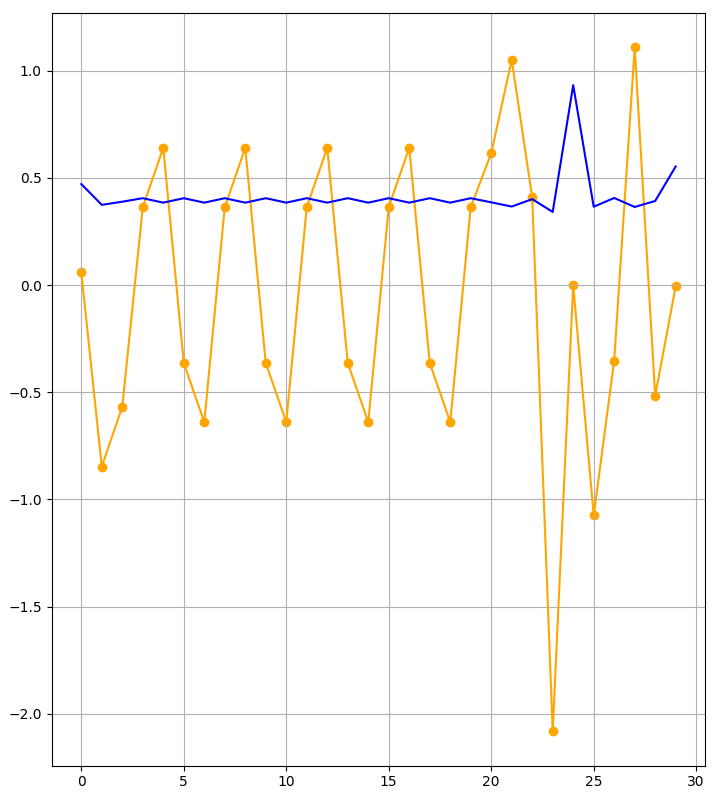
\includegraphics[width=50mm,height=45mm]{Graphics/patternDetected1D.png}
\caption{Vector $cD$ obtenido tras aplicar la DST (naranja) y la medida de similaridad con $\alpha=0.1$ (azul).}
\end{figure}

\par Como se cumple que:
\begin{eqnarray}
cD(n)=0&\Leftrightarrow& D(f\ast\tilde{v})(n)=0\nonumber\\
&\Leftrightarrow&(f\ast\tilde{v})(2n)=0\nonumber\\
&\Leftrightarrow&\sum_{m=0}^{N-1}v(m)f(2n-m)=0,\nonumber
\end{eqnarray}
entonces, si $cD(n)=0$ el patr\'on se encuentra contenido en $f$ en el intervalo $[2n-N+1,2n]$, por tanto, tomando $n=24$, se cumple que $2n-N+1=41$ es la posici\'on exacta en la que comienza el patr\'on dentro de la se\~nal.

\par Como parte del an\'alisis del programa se generaron varios patrones de forma aleatoria con dimensi\'on tambi\'en variable y se insertaron dentro de una se\~nal en una posici\'on aleatoria con una probabilidad de $0.5$. Sin embargo, el patr\'on fue detectado satisfactoriamente en el $100\%$ de los casos que aparec\'ia, al igual que la detecci\'on de la ausencia en el $100\%$ de los casos en los que no se incluy\'o el patr\'on en la se\~nal.\\

\par Como un segundo experimento, se generaron $676$ casos de prueba con patr\'on aleatorio e inclusi\'on aleatoria en la se\~nal, pero esta vez con un ruido en el orden $10^{-3}$.  La Figura 3.8 muestra los gr\'aficos de precisi\'on y recobrado del algoritmo durante el proceso de detecci\'on de la presencia o no del patr\'on en dependencia del umbral usado para la medida de similiaridad.

\begin{figure}[h]
\center
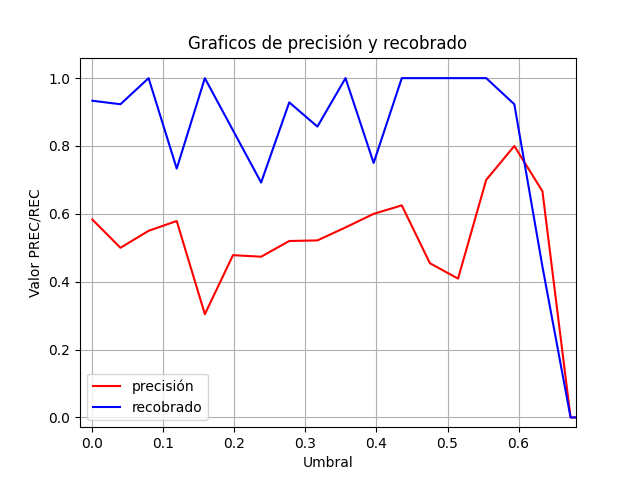
\includegraphics[scale=.45]{Graphics/PrecRec1D.png}
\caption{Precisi\'on y Recobrado del algoritmo de una dimensi\'on para distintos valores del umbral usando la mediada $\mathbb{S}$.}
\end{figure}

\par Note que, aun con la presencia de ruido en el patr\'on dentro de la se\~nal, se muestra un valor de precisi\'on y recobrado aceptable. Como un \'ultimo experimento, se usaron otras bases wavelets (las mencionadas al final de la secci\'on 1.1.3) para intentar detectar el patr\'on sin \'exito alguno. La raz\'on de esto se debe a que ninguna de estas wavelets tiene en cuenta el patr\'on que se desea localizar, por tanto, no se puede esperar obtener un comportamiento distinto para distintos casos de patrones que se incluyan en una se\~nal.

\section{Algoritmo de reconocimiento en dos dimensiones}

\par El problema principal, es crear una base wavelet que permita reconocer anomal\'ias en una mamograf\'ia digital. Para ello, tanto la mamograf\'ia como la anomal\'ia son representadas como im\'agenes con la particularidad de que esta \'ultima debe tener iguales proporciones de ancho y altura. Estas im\'agenes que representan los datos a procesar se encuentran en formato \texttt{.dcm}, tambi\'en conocido como im\'agenes DICOM. Este es un formato internacional que se desarrolló con el fin de almacenar las imágenes del cuerpo tomadas con equipos de imágenes médicas. Incluye imágenes de resonancia magnética y tomografía por ordenador, imágenes de ultrasonido, mamograf\'ias, entre otras, en una escala real. DCM también almacena la información del paciente en los metadatos, que forman parte de un único archivo.\\

\par En el software desarrollado se emplea la biblioteca \textit{Pydicom} [\cite{15}], creada espec\'ificamente para el trabajo con archivos de tipo \texttt{dcm}. Sup\'ongase que se desea leer primeramente la imagen de la anomal\'ia que a su vez constituye el patr\'on, usando \textit{pydicom} ser\'ia tan simple como ejecutar:\\
\begin{lstlisting}[caption=Leer una imagen .dcm., label=pydicom-read]
ds = pydicom.dcmread(path, force=True)
\end{lstlisting}
con lo cual se lee la imagen de la direcci\'on \texttt{path} y se almacena en \texttt{ds} como un archivo de tipo \texttt{pydicom.FileDataset}. De aqu\'i, lo m\'as relevante, es el valor de \texttt{ds.pixel\_array}, que contiene la matriz de valores de los p\'ixeles de la mamograf\'ia.\\

\par El siguiente paso, es crear el sistema de ecuaciones no lineales. Y aqu\'i una nota muy importante, aunque el m\'etodo de Newton usado con Runge-Kutta mostr\'o mejores resultados en el caso de una dimensi\'on, al incluir dos ecuaciones nuevas con una cantidad de $N^2$ t\'erminos, el m\'etodo de Newton comienza a presentar dificultades para resolver el sistema, mientras que por otro lado, Gekko muestra un buen desempe\~no con el aumento de t\'erminos, esto se debe a que dicha biblioteca posee su propio m\'etodo de representar los datos. Entonces, dado que ambos m\'etodos (Gekko y Runge-Kutta) requieren una representaci\'on distinta de los datos, existen dos formulaciones del modelo en el programa. El primero de ellos (Runge-Kutta) usa la funci\'on multivariable como la funci\'on a la cual se le quiere hallar la ra\'iz y el jacobiano del sistema. Para esto se crearon dos funciones: \texttt{func} y \texttt{jac} que retornan la evaluaci\'on de la funci\'on multivariable y el jacobiano en un punto dado, respectivamente. Para mejorar la eficiencia del programa, se plante\'o el sistema en forma matricial usando la biblioteca de Python: \textit{numpy} [\cite{14}], de esta forma evaluar cada funci\'on en un valor del dominio se transforma en operaciones entre matrices \textit{numpy}, que se realizan en un tiempo mucho menor en comparaci\'on a las operaciones con matrices en Python.
\par Por su parte, Gekko usa las ecuaciones en su representaci\'on algebraica, esto es plantear las ecuaciones tal y como se plantearon en (1.1)-(1.5), una vez hecho se definen las opciones de resoluci\'on del sistema y, por \'ultimo, se invoca al m\'etodo \texttt{solve()} para encontrar la soluci\'on.\\

\par Tras construir la wavelet con el banco de filtro hallado, se procede a cargar la imagen de prueba usando \textit{pydicom} como se muestra en el ejemplo de c\'odigo~\ref{pydicom-read}. De la imagen se extrae la matriz de valores de los p\'ixeles y se le aplica la transformada wavelet de dos dimensiones.
\par N\'otese algo muy importante, en las mamograf\'ias digitales predominan los valores 0, que representan el color negro en la escala de grises, al aplicar la transformada de wavelets en dos dimensiones usando \textit{PyWavelets}, en alg\'un punto se calcula la convoluci\'on entre el filtro y una secuencia de ceros en la imagen, lo cual va a resultar en un valor igual a cero en la matriz de detalle. Dado que se usa la cercan\'ia a este valor como medida de similaridad entre el patr\'on y el fragmento de la muestra, podr\'ia representar un problema, llegando a producir un gran n\'umero de falsos positivos.
\par Para evitar este inconveniente se calcula la transformada wavelet de forma manual, as\'i, si en alg\'un punto se calcula la convoluci\'on entre el vector $\tilde{v}$ del filtro y una secuencia de al menos $\frac{N^2}{4}$ ceros, no se considera el resultado obtenido como posible ocurrencia del patr\'on.\\

\par Al aplicar entonces la transformada wavelet se obtienen las matrices \texttt{cA}, \texttt{cH}, \texttt{cV} y \texttt{cD}. De ellas se toma la \'ultima y se realiza la b\'usqueda de ceros que indiquen la ocurrencia del patr\'on. Sup\'ongase que se encuentra una posible ocurrencia del patr\'on en $(i,j)$, realizando el mismo an\'alisis que en una dimensi\'on, se tiene:
\begin{eqnarray}
cD(i,j)=0&\Leftrightarrow&D(img\ast\tilde{w}_{0,0})(i,j)=0\nonumber\\
&\Leftrightarrow&(img\ast\tilde{w}_{0,0})(2i,2j)=0\nonumber\\
&\Leftrightarrow&\sum_{n=0}^{N-1}\sum_{m=0}^{N-1}\tilde{w}_{0,0}(n,m)img(2i-n,2j-m)=0,\nonumber
\end{eqnarray}
cuyo resultado indica la ocurrencia del patr\'on entre $(2i-N+1,2j-N+1)$ y $(2i,2j)$.

\par Un punto muy importante que se tiene en cuenta es la ocurrencia del patr\'on en una imagen con ruido. En estos casos es casi imposible lograr una medida $\mathbb{S}$ cercana a la unidad, por esta raz\'on se emplea un umbral de detecci\'on, de esta forma, cualquier valor en la medida $\mathbb{S}$ que sobrepase este umbral es considerada una ocurrencia del patr\'on, mientras que, de quedar por debajo, se considera que el patr\'on no se localiz\'o en la posici\'on actual.\\

\par Para analizar el funcionamiento del algoritmo se mostrar\'a un ejemplo con im\'agenes. Suponga que se desea reconocer la ocurrencia de una letra (digamos \texttt{c}, ver Figura~\ref{img-ejemplo}) en una lista de palabras:

\begin{figure}[h]
\center
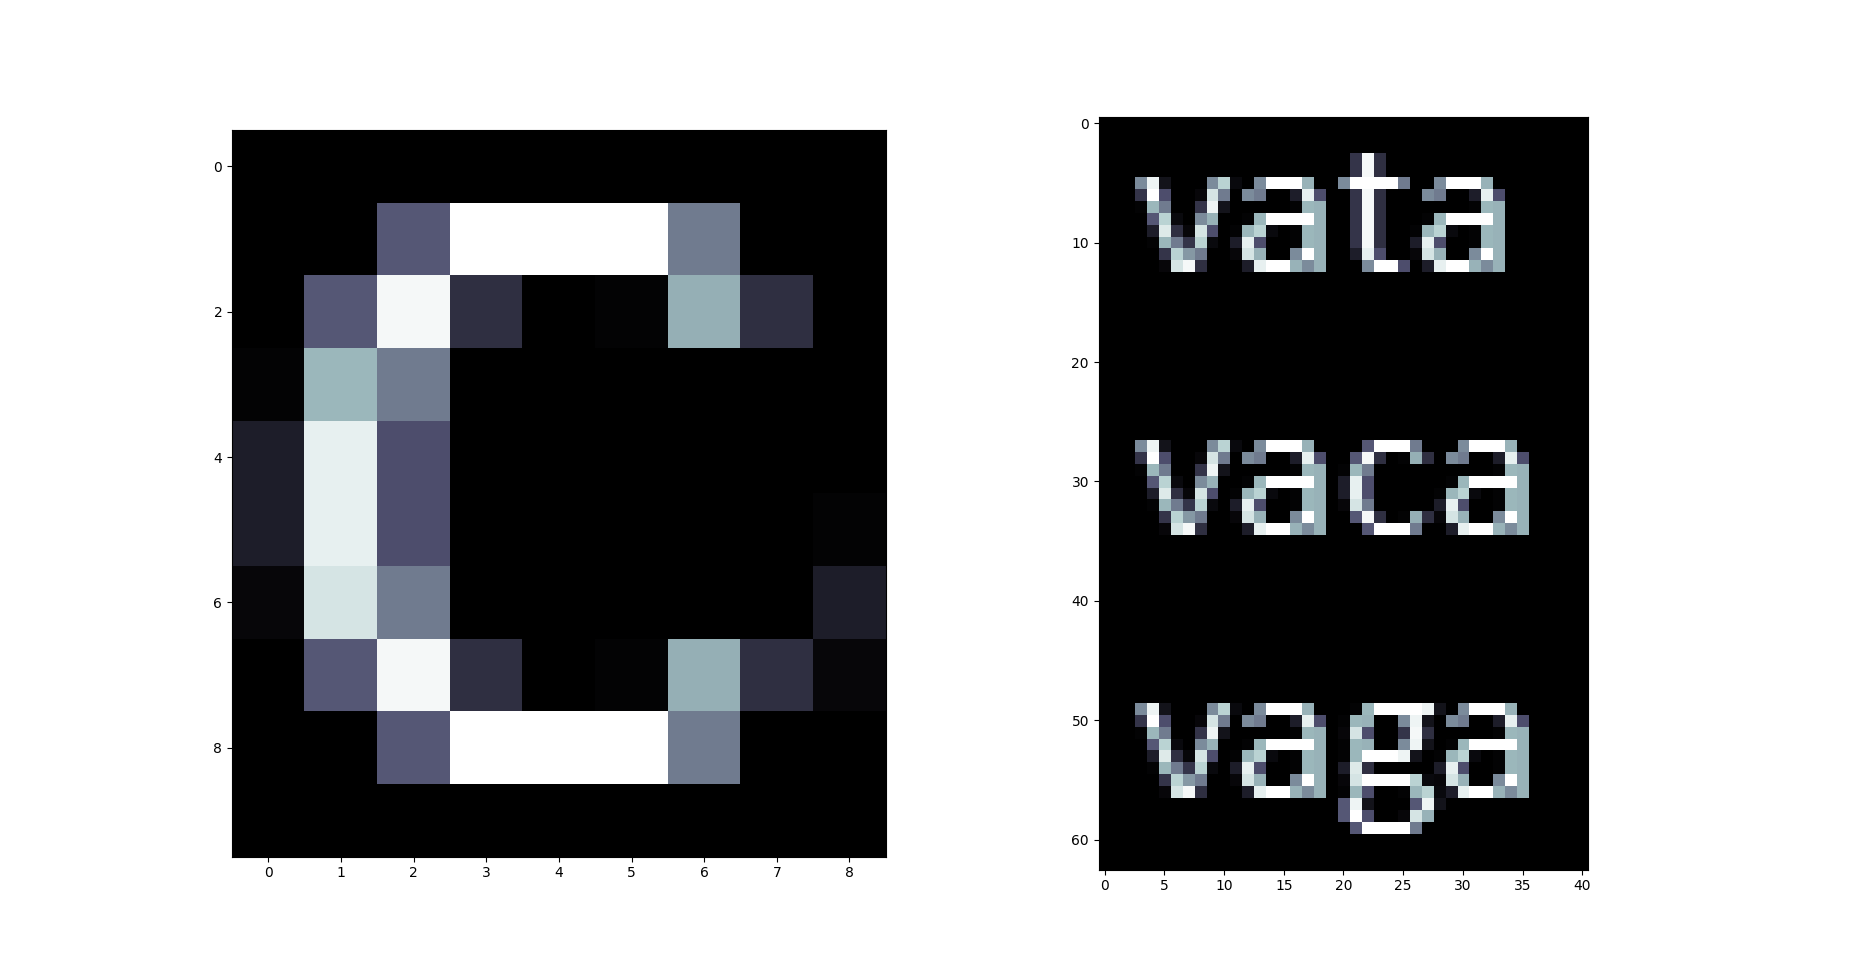
\includegraphics[scale=.2]{Graphics/cWordList.png}
\caption{Ejemplo de un patr\'on y una imagen de prueba.}
\label{img-ejemplo}
\end{figure}

\par Para este caso se toma $N=8$ como la dimensi\'on de los vectores del filtro. Tras leer la imagen con \textit{PyWavelets}, se obtiene la siguiente representaci\'on matricial:
\begin{scriptsize}
\begin{eqnarray}
m&=&\left[\begin{array}{rrrrrrrrr}
0&0&0&0&0&0&0&0&0\\
0&0&0.0015&0.0039&0.0039&0.0039&0.002&0&0\\
0&0.0015&0.0038&0.0008&0&0.0001&0.0026&0.0008&0\\
0.0001&0.0027&0.002&0&0&0&0&0&0\\
0.0005&0.0036&0.0014&0&0&0&0&0&0\\
0.0005&0.0036&0.0014&0&0&0&0&0&0.0001\\
0.0001&0.0034&0.002&0&0&0&0&0&0.0005\\
0&0.0015&0.0038&0.0008&0&0.0001&0.0026&0.0008&0.0001\\
0&0&0.0015&0.0039&0.0039&0.0039&0.002&0&0\\
0&0&0&0&0&0&0&0&0
\end{array}\right].\nonumber
\end{eqnarray}
\end{scriptsize}

\par Con los valores de esta matriz se construyen las ecuaciones de detecci\'on y junto con el resto de las condiciones se forma el sistema de ecuaciones. A la hora de resolverlo se usa primeramente una aproximaci\'on inicial a la r\'aiz proporcionado por el m\'etodo de Runge-Kutta. Los valores $x_0$ son generados de forma aleatoria y por tanto la ra\'iz encontrada en cada ejecuci\'on podr\'ia cambiar. Por ejemplo, en este caso, antes de aplicar Runge-Kutta:
\begin{eqnarray}
x_0&=&(0.773,0.7211,0.382,0.0948,0.0963,0.963,0.2968,0.1797),\nonumber
\end{eqnarray}
mientras que, al aplicar Runge-Kutta se tiene:
\begin{eqnarray}
x_{\ast}&=&(-0.0607,-2.5645,4.3419,14.4576,-0.7601,-21.0409,-2.3254,-8.2964),\nonumber
\end{eqnarray}
el valor de $x_{\ast}$ es usado entonces como valor inicial al aplicar el m\'etodo de \textit{Gekko}. Tras resolver el sistema nuevamente se obtiene:
\begin{eqnarray}
v&=&(0.0061,-0.0121,-0.0813,-0.0222,0.6232,-0.7612,0.141,0.0708).\nonumber
\end{eqnarray}
\par A partir del valor de $v$ obtenido, se calculan el resto de los vectores que conformar\'an el banco de filtros:
\begin{eqnarray}
u&=&(-0.0121,0.0061,0.0708,-0.141,-0.7612,-0.6232,-0.0222,0.0813),\nonumber\\
\tilde{v}&=&(0.0061,0.0708,0.141,-0.7612,0.6232,-0.0222,-0.0813,-0.0121),\nonumber\\
\tilde{u}&=&(-0.0121,0.0813,-0.0222,-0.6232,-0.7612,-0.141,0.0708,0.0061),\nonumber
\end{eqnarray}
con el cual se construye la shapelet.\\

\begin{figure}[h]
\center
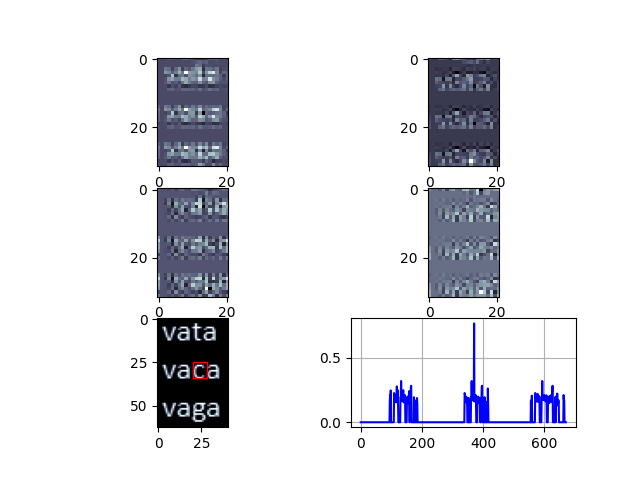
\includegraphics[scale=.7]{Graphics/CDetect.png}
\caption{Imagenes de aproximaci\'on, detalles horizontales, detalles verticales, detalles (com\'unmente llamados diagonales), imagen con el patr\'on se\~nalado y medida $\mathbb{S}$, en ese orden.}
\label{c-detected}
\end{figure}

\par Para el paso de an\'alisis de la imagen en busca de la ocurrencia del patr\'on, se carga el archivo de la misma a partir de su direcci\'on tal como se muestra en el Ejemplo de c\'odigo~\ref{pydicom-read}. Una vez se tiene la forma matricial de la imagen de muestra, se determina la transformada wavelet de dos dimensiones usando la shapelet creada. La Figura~\ref{c-detected} muestra las im\'agenes obtenidas tras aplicar las transformadas junto con los valores de la medida $\mathbb{S}$ para $\alpha=0.1$ aplicada a la matriz \texttt{cD}.

\par Como se puede apreciar hay una amplia diferencia entre la medida $\mathbb{S}$ del punto en el que coincide el patr\'on y el resto de los puntos. Este ejemplo muestra un buen comportamiento del algoritmo, por ello se pasar\'a a analizar que ocurrir\'ia en casos m\'as complejos como es el de detectar tumores en mamograf\'ias.\\

\par Para el siguiente ejemplo, se tom\'o una anomal\'ia y, aplicando la transformada wavelet de Haar, se le redujo la dimensi\'on hasta tener proporciones menores o iguales que una imagen de $26\times 26$ p\'ixeles. La raz\'on se debe a la efectividad mostrada por los m\'etodos de resoluci\'on de sistemas de ecuaciones no lineales ante un aumento del n\'umero de variables. Posteriormente, se determin\'o la shapelet asociada al patr\'on. Luego, se tom\'o una mamograf\'ia digital con el tumor, se redujo sus dimensiones usando el mismo m\'etodo que para el patr\'on un n\'umero igual de veces y, se le aplic\'o la transformada usando la shapelet antes creada. La Figura~\ref{detect-anomalia} muestra los resultados obtenidos en el proceso de detecci\'on.

\begin{figure}[h]
\center
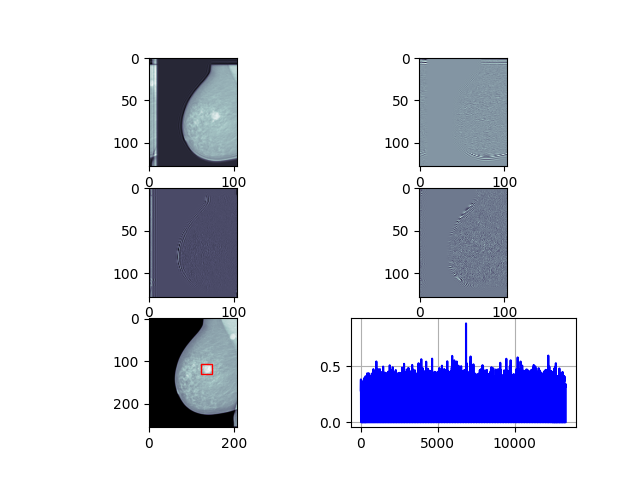
\includegraphics[scale=.7]{Graphics/MamografiaDetect.png}
\caption{Resultados obtenidos en el proceso de detecci\'on de la anomal\'ia en la mamograf\'ia.}
\label{detect-anomalia}
\end{figure}

\par En un segundo ejemplo, se muestra una mamograf\'ia con una anomal\'ia de distinto tama\~no a la anterior y el resultado que se obtiene al ejecutar el algoritmo. Tal como se puede observar en la Figura~\ref{detect-anomalia-piece}, el algoritmo detecta la ocurrencia del patr\'on con una similitud de m\'as del $40\%$, sin embargo, la anomal\'ia es mayor a la del patr\'on empleado, por lo que solo es posible reconocer una peque\~na parte de esta.

\begin{figure}[h]
\center
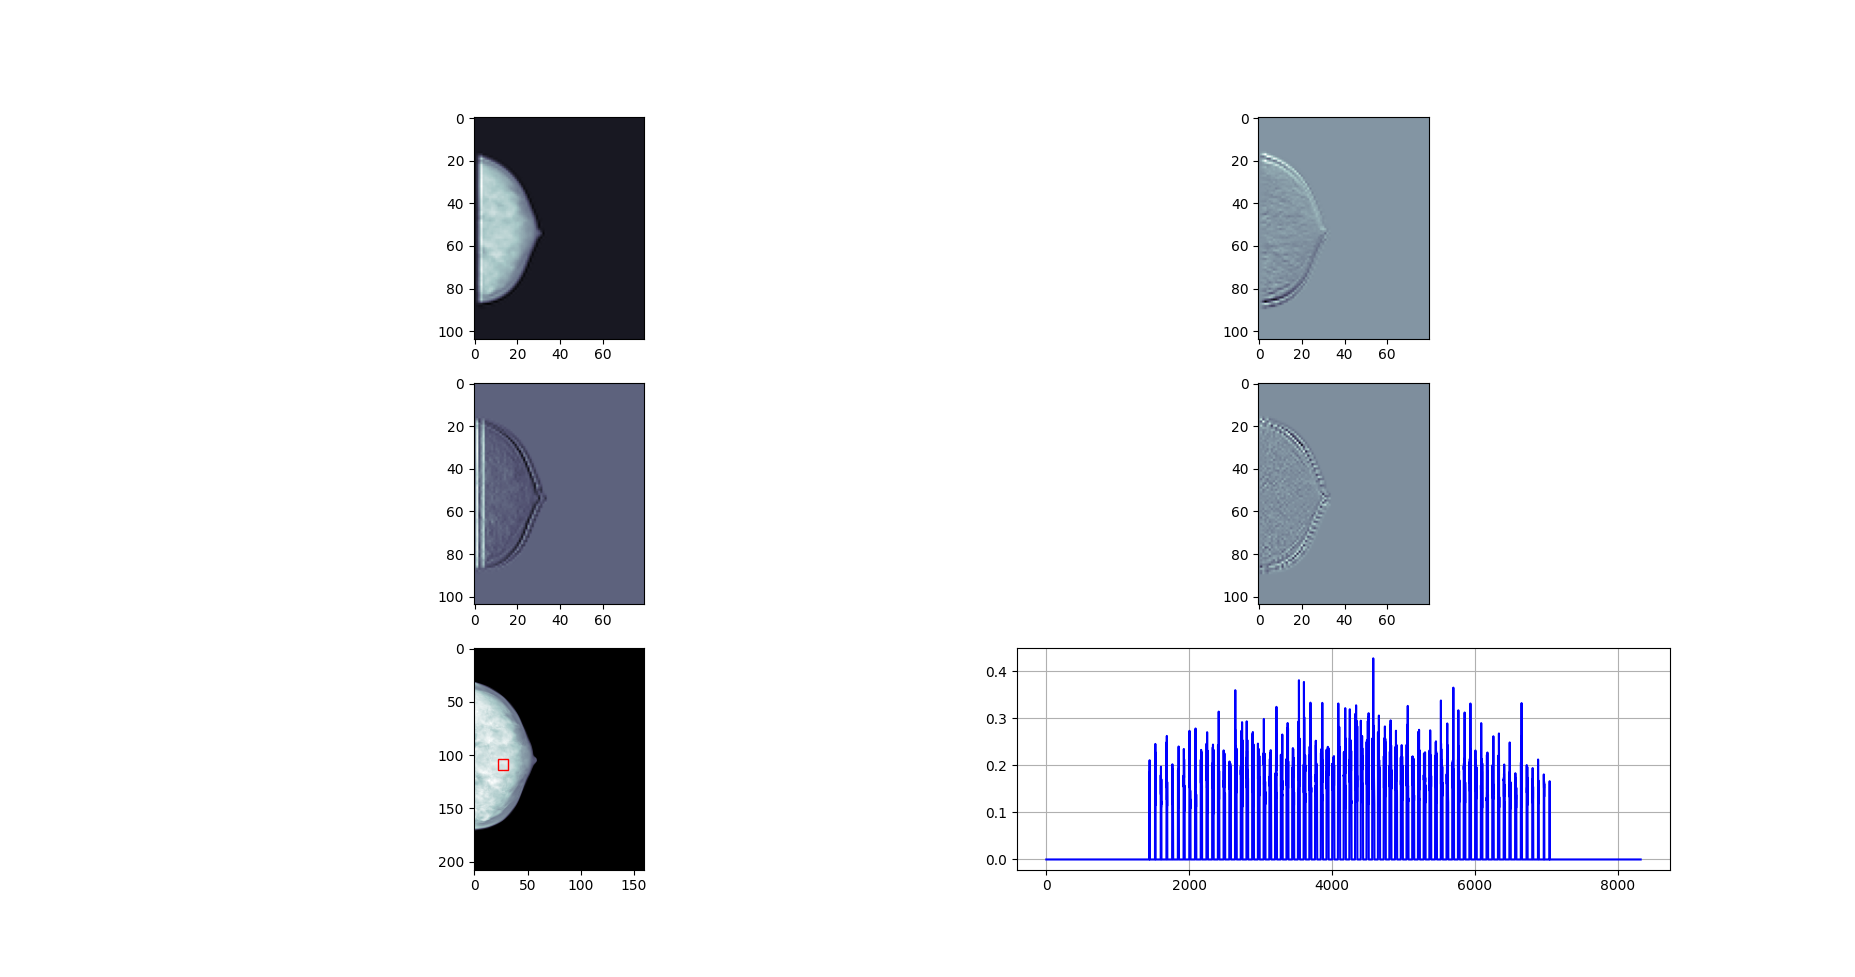
\includegraphics[scale=.32]{Graphics/MamografiaDetectPiece.png}
\caption{Resultados obtenidos en el proceso de detecci\'on de la anomal\'ia irregular en la mamograf\'ia.}
\label{detect-anomalia-piece}
\end{figure}

\par Como tercer ejemplo, se tom\'o una mamograf\'ia sin anomal\'ias, pero, debido a las caracter\'isticas de la imagen, el algoritmo produjo un falso positivo como se muestra en la Figura~\ref{detect-anomalia-fail}. La textura de una im\'agen puede variar en dependencia del equipo con el cual se haya tomado la muestra y, puede repercutir positiva o negativamente en el proceso de reconocimiento.

\begin{figure}[h]
\center
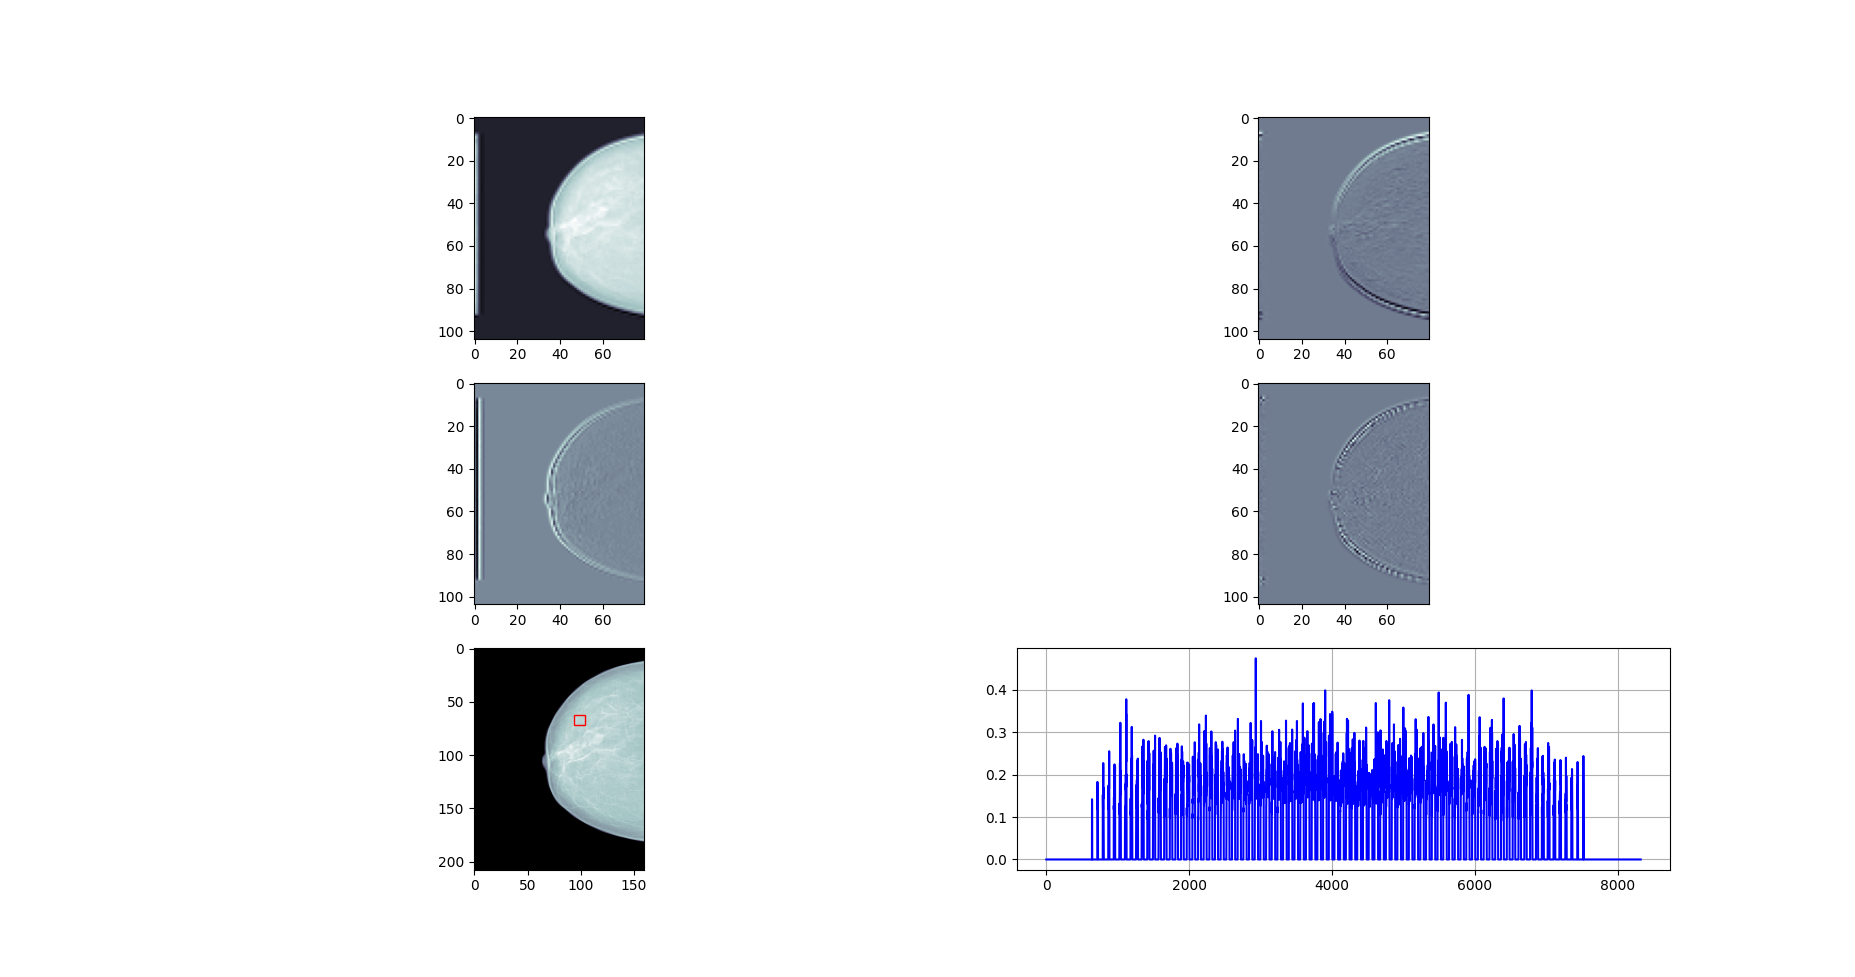
\includegraphics[scale=.32]{Graphics/MamografiaDetectFail.png}
\caption{Resultados obtenidos en el proceso de reconocimiento en una imagen sin anomal\'ias.}
\label{detect-anomalia-fail}
\end{figure}

\par Para poner a prueba el algoritmo, se tom\'o una colecci\'on de mamograf\'ias digitales tanto de personas sanas, como de personas con c\'ancer y con presencia de un posible tumor. Se tom\'o un patr\'on de una anomal\'ia, se cre\'o la sheplet correspondiente y, posteriormente, se ejecut\'o el algoritmo para cada imagen de muestra. La Figura~\ref{prec-rec-2d} muestra los valores de precisi\'on y recobrado para un aumento de los casos de prueba.

\begin{figure}[h]
\center
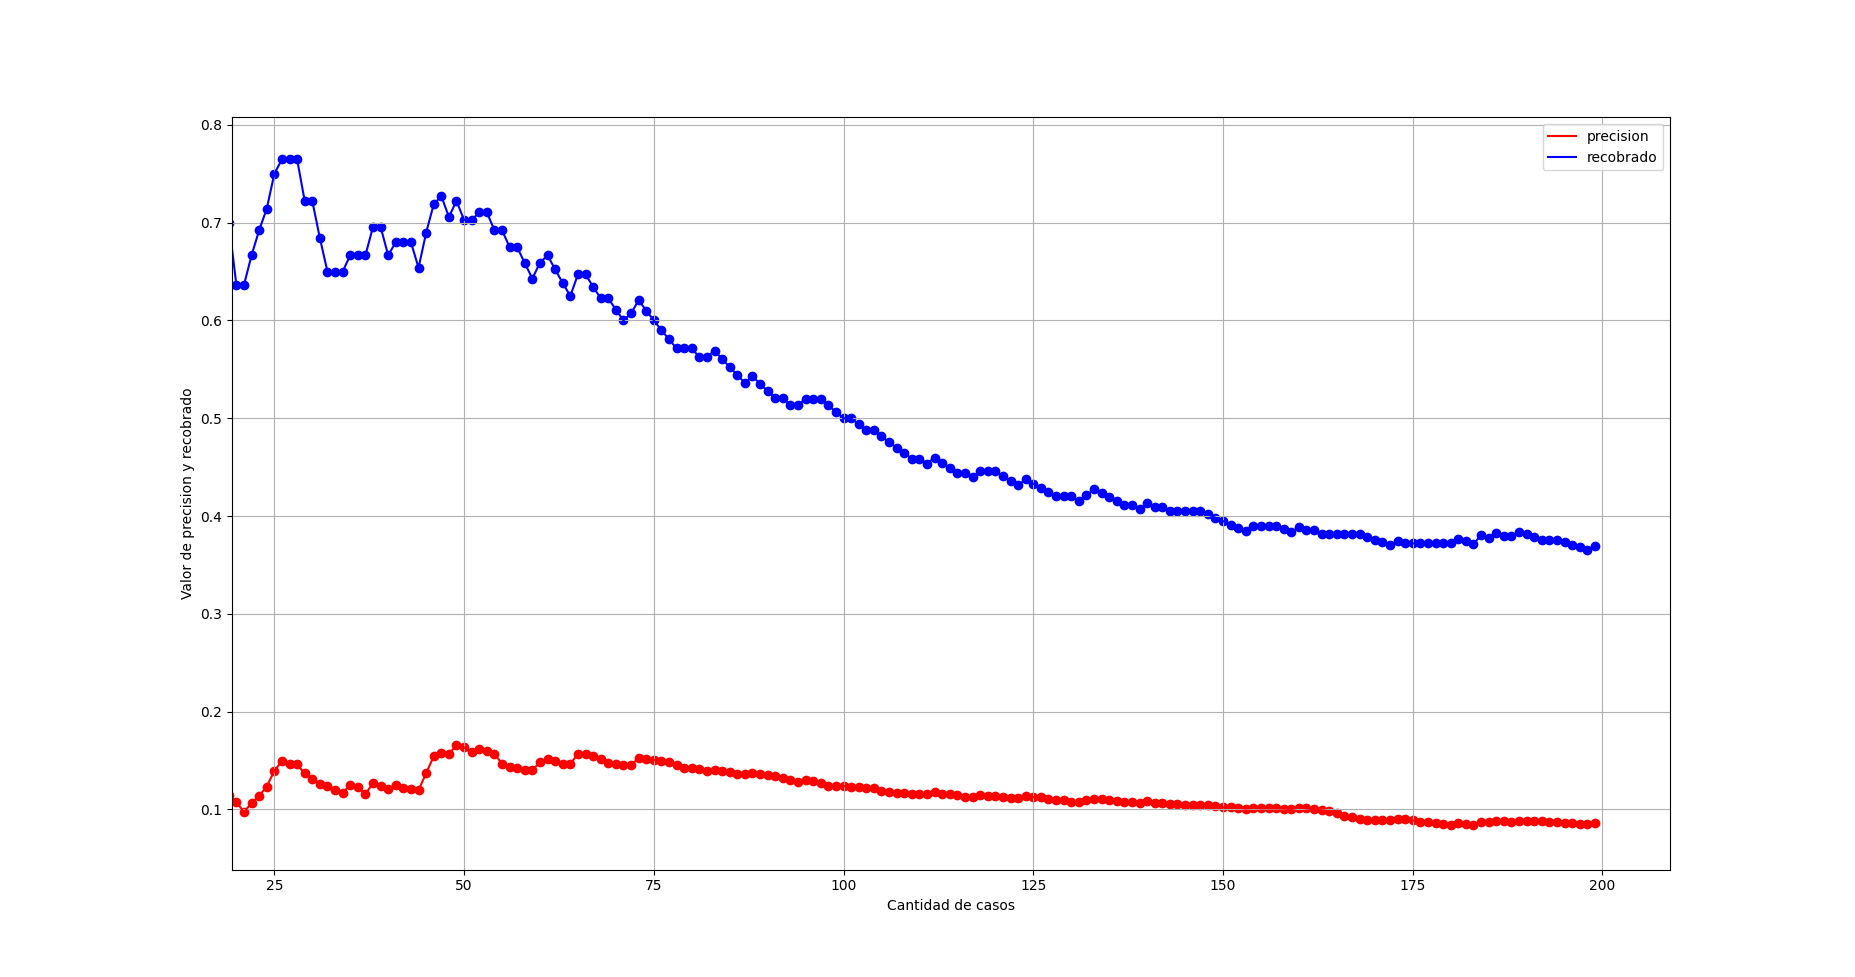
\includegraphics[scale=.25]{Graphics/PrecRec2D.png}
\caption{Valores de precisi\'on y recobrado obtenidos durante el aumento de los datos procesados, de una colecci\'on de $200$ mamograf\'ias.}
\label{prec-rec-2d}
\end{figure}

\par El proceso de detectar un tumor en una mamograf\'ia se ve afectado por varios factores: forma del patr\'on, tama\~no, opacidad, todos f\'acilmente clasificados como ruido en el proceso de reconocimiento. Para lidiar con estos problemas, ser\'ia necesario incluir en el proceso de construcci\'on de la shepelet, un peso distinto a los valores de la imagen tomada como patr\'on que no pertenezcan a la anomal\'ia; al igual que con la wavelet de Daubechies, ser\'ia necesario crear una familia de wavelets para distintos valores de $N$ que permita detectar patrones con proporci\'on distinta y, antes de realizar el proceso de reconocimiento, normalizar tanto al patr\'on como a la imagen.\\

\par Este software fue creado basado en la teor\'ia antes expuesta, por lo que solo se encuentra en su fase experimental. Mejorando varios aspectos como la resoluci\'on del sistema, la representaci\'on de las im\'agenes y la detecci\'on efectiva del patr\'on, podr\'ia convertirse en una muy buena herramienta para identificar anomal\'ias y llegar incluso a salvar vidas con la detecci\'on temprana del c\'ancer de mama.